\documentclass[aspectratio=169,11pt]{beamer}

% Metropolis theme - modern and clean
\usetheme{metropolis}

% Custom colors
\definecolor{iubblue}{RGB}{0,82,147}
\definecolor{mDarkTeal}{RGB}{23,55,94}

\setbeamercolor{palette primary}{bg=iubblue}
\setbeamercolor{frametitle}{bg=iubblue}
\setbeamercolor{progress bar}{fg=iubblue,bg=iubblue!20}
\setbeamercolor{alerted text}{fg=iubblue}

% Progress bar on each frame
\metroset{progressbar=frametitle}
\metroset{numbering=fraction}
\metroset{block=fill}

% Add space between frametitle bar and slide content
\addtobeamertemplate{frametitle}{}{\vspace*{0.4cm}}

% Packages
\usepackage[utf8]{inputenc}
\usepackage[T1]{fontenc}
\usepackage{lmodern}
\usepackage{amsmath,amssymb,amsthm}
\usepackage{physics}
\usepackage{graphicx}
\graphicspath{{./}{figures/}}
\usepackage{tikz}
\usepackage{pgfplots}
\pgfplotsset{compat=1.18}
\usetikzlibrary{arrows.meta,positioning,calc,decorations.pathreplacing}
\usepackage{booktabs}
\usepackage{hyperref}

% Bibliography
\usepackage[style=phys,backend=biber,sorting=none,maxbibnames=3]{biblatex}
\addbibresource{references.bib}

% Custom commands
\newcommand{\avg}[1]{\left\langle#1\right\rangle}
\newcommand{\Hsys}{\mathcal{H}_{\mathrm{sys}}}
\newcommand{\Henv}{\mathcal{H}_{\mathrm{env}}}

% Suppress harmless hyperref/beamer \translate bookmark warning (PDF output is correct)
% This is a known beamer issue: \translate is not PDF-string-safe
\makeatletter
\g@addto@macro\pdfstringdefPreHook{%
  \let\translate\@firstofone
}
\makeatother

% Title information
\title[Page Curve Entanglement]{Page-Curve-Like Entanglement Dynamics in Many-Body Quantum Systems}
\subtitle{A Study of a Free Fermionic Model}
\author[P. Bhakta]{Prosanto Bhakta}
\institute[IUB]{Department of Physical Sciences, Independent University Bangladesh}
\date{February 2026}

% Logo (uncomment if you have a logo)
% \logo{
\includegraphics[height=1cm]{iub_logo.png}}

\begin{document}

% Title slide
\begin{frame}[plain]
    \titlepage
\end{frame}

% Outline
\begin{frame}{Outline}
    \tableofcontents
\end{frame}

%=============================================================================
\section{Introduction}
%=============================================================================

\begin{frame}{Motivation: The Page Curve}
    \begin{columns}
        \begin{column}{0.56\textwidth}
            \textbf{Black-hole information problem:}
            \begin{itemize}
                \item Hawking radiation entangles emitted and remaining degrees of freedom
                \item Under unitary evolution, entropy cannot grow forever
                \item Expected trajectory: rise $\rightarrow$ peak $\rightarrow$ fall
            \end{itemize}

            \vspace{0.2cm}
            \textbf{Thesis question:} can the same structure appear in a simple solvable many-body model?
            \vspace{0.05cm}
            {\footnotesize Refs.~\cite{Hawking1975,Page1993,Penington2020,Almheiri2020}}
        \end{column}
        \begin{column}{0.44\textwidth}
            \begin{center}
                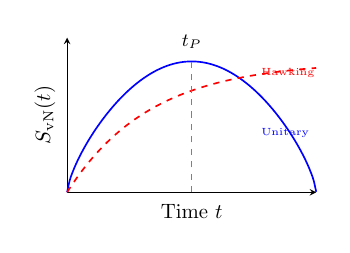
\begin{tikzpicture}[scale=0.75]
                    \begin{axis}[
                        xlabel={Time $t$},
                        ylabel={$S_{\mathrm{vN}}(t)$},
                        xmin=0, xmax=10,
                        ymin=0, ymax=1.3,
                        axis lines=left,
                        width=5.8cm,
                        height=4.2cm,
                        xtick=\empty,
                        ytick=\empty,
                        clip=false,
                    ]
                    % Page curve (unitary)
                    \addplot[thick, blue, smooth, samples=100, domain=0:10] 
                        {1.1*sin(deg(x*3.14159/10))^0.7};
                    % Hawking (thermal) — monotonic
                    \addplot[thick, red, dashed, smooth, samples=100, domain=0:10]
                        {1.1*(1 - exp(-0.3*x))};
                    \node[above] at (axis cs:5,1.15) {\small $t_P$};
                    \draw[dashed, gray] (axis cs:5,0) -- (axis cs:5,1.1);
                    \node[right, blue] at (axis cs:7.5,0.5) {\tiny Unitary};
                    \node[right, red] at (axis cs:7.5,1.0) {\tiny Hawking};
                    \end{axis}
                \end{tikzpicture}
            \end{center}
        \end{column}
    \end{columns}
\end{frame}

\begin{frame}{Context \& Objectives}
\small
    \textbf{Page curve beyond black holes:}
    \begin{itemize}\setlength{\itemsep}{1pt}
        \item This thesis follows Kehrein (2024)~\cite{Kehrein_2024}: \alert{exactly solvable} free-fermion model
        \item \textbf{Advantage:} full analytical control + numerical verification in a single model
    \end{itemize}

    \vspace{0.15cm}
    \textbf{Goal:} Establish Page-curve-like entanglement dynamics in a solvable open free-fermion model

    \vspace{0.1cm}
    \begin{enumerate}\setlength{\itemsep}{1pt}
        \item Define the model and initial state (system full, environment empty)
        \item Derive weak-coupling analytical dynamics via resonant level model factorization
        \item Compute $S_{\mathrm{vN}}(t)$ numerically using correlation matrices (Peschel formalism)
        \item Compare analytics and numerics; test universal scaling versus emitted fraction
    \end{enumerate}
\end{frame}

\begin{frame}{Methodology Overview}
    \begin{center}
    \resizebox{0.95\textwidth}{!}{%
    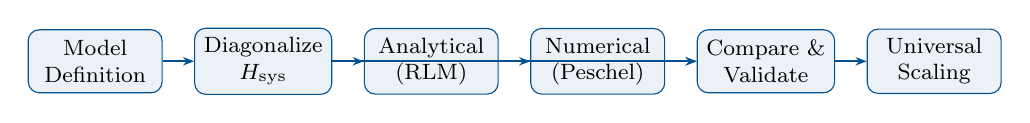
\begin{tikzpicture}[
        box/.style={draw=iubblue, fill=iubblue!8, rounded corners=4pt, 
                     minimum width=1.7cm, minimum height=0.8cm, align=center, 
                     font=\footnotesize},
        arr/.style={-{Stealth[length=4pt]}, thick, iubblue},
        node distance=0.4cm
    ]
    \node[box] (model) {Model\\Definition};
    \node[box, right=of model] (diag) {Diagonalize\\$H_{\mathrm{sys}}$};
    \node[box, right=of diag] (ana) {Analytical\\(RLM)};
    \node[box, right=of ana] (num) {Numerical\\(Peschel)};
    \node[box, right=of num] (comp) {Compare \&\\Validate};
    \node[box, right=of comp] (univ) {Universal\\Scaling};
    
    \draw[arr] (model) -- (diag);
    \draw[arr] (diag) -- (ana);
    \draw[arr] (diag) -- (num);
    \draw[arr] (ana) -- (comp);
    \draw[arr] (num) -- (comp);
    \draw[arr] (comp) -- (univ);
    \end{tikzpicture}%
    }
    \end{center}
    
    \vspace{0.3cm}
    \begin{columns}
        \begin{column}{0.5\textwidth}
            \textbf{Analytical path:}
            \begin{itemize}
                \item Resonant level model (RLM) factorization
                \item Exponential decay in each mode
                \item Continuum limit $\to$ universal form
            \end{itemize}
        \end{column}
        \begin{column}{0.5\textwidth}
            \textbf{Numerical path:}
            \begin{itemize}
                \item Correlation matrix evolution
                \item Extract system block, diagonalize
                \item Entropy from eigenvalues $\{\nu_k\}$
            \end{itemize}
        \end{column}
    \end{columns}
\end{frame}

%=============================================================================
\section{Theoretical Background}
%=============================================================================

\begin{frame}{Density Matrix and Reduced States}
    \textbf{Density matrix} --- the most general state description:
    \[
        \rho = \sum_i p_i\ket{\psi_i}\bra{\psi_i}, \qquad \Tr(\rho)=1, \quad \rho \geq 0
    \]
    \begin{itemize}
        \item \textbf{Pure state:} $\rho = \ket{\psi}\bra{\psi}$, $\Tr(\rho^2) = 1$
        \item \textbf{Mixed state:} statistical mixture, $\Tr(\rho^2) < 1$
        \item Expectation values: $\langle A \rangle = \Tr(\rho A)$
    \end{itemize}

    \vspace{0.2cm}
    \textbf{Bipartite system:} $\mathcal{H} = \mathcal{H}_A \otimes \mathcal{H}_B$
    \[
        \rho_A = \Tr_B(\rho_{AB}) \qquad \text{(partial trace over } B \text{)}
    \]
    The reduced density matrix $\rho_A$ reproduces \emph{all} measurements on $A$ alone:
    $\langle M_A \rangle = \Tr_A(\rho_A M_A)$.
\end{frame}

\begin{frame}{What is Entanglement?}
    A bipartite pure state $\ket{\Psi} = \sum_{n,m} C_{nm}\ket{\psi_n}_A \otimes \ket{\phi_m}_B$ is:
    \begin{itemize}
        \item \textbf{Separable} if $C_{nm} = c_{A,n}\, c_{B,m}$ (product state)
        \item \textbf{Entangled} if no such factorization exists
    \end{itemize}

    \vspace{0.1cm}
    \textbf{Key consequence:} for entangled states, $\rho_A = CC^\dagger$ is a \alert{mixed state}, even though $\rho_{AB}$ is pure.

    \vspace{0.1cm}
    \textbf{Bell state example:}
    \[
        \ket{\Psi} = \tfrac{1}{\sqrt{2}}(\ket{0}_A\ket{1}_B + \ket{1}_A\ket{0}_B) \quad \Longrightarrow \quad \rho_A = \tfrac{1}{2}\mathbb{I}_A
    \]
    \begin{itemize}
        \item Maximally entangled: subsystem is maximally mixed
        \item Complete information about $A$ resides in correlations with $B$
    \end{itemize}
\end{frame}

\begin{frame}{Entanglement Entropy}
\small
    \textbf{Von Neumann entropy:} $S_{\mathrm{vN}}(\rho) = -\Tr(\rho \ln \rho) = -\sum_n p_n \ln p_n$, where $\{p_n\}$ are eigenvalues of $\rho$.

    \textbf{Entanglement entropy} $\equiv$ von Neumann entropy of the reduced state:
    \[
        \boxed{S_A = -\Tr_A(\rho_A \ln \rho_A) = S_B}
    \]

    \textbf{Properties:}
    \begin{itemize}\setlength{\itemsep}{1pt}
        \item $S_A = 0$ iff $\ket{\Psi}$ is a product state; $S_A = \ln(\dim\mathcal{H}_A)$ for maximally entangled states
        \item Bell state: $S = \ln 2 \approx 0.693$
        \item $S_A = S_B$ guaranteed by \textbf{Schmidt decomposition}
    \end{itemize}

    \textbf{Physical meaning:} uncertainty about $A$ caused purely by quantum correlations with $B$ --- not classical ignorance.
\end{frame}

\begin{frame}{Second Quantization for This Problem}
\small
    \textbf{Fermionic operators} --- canonical anticommutation relations (CAR):
    \[
        \{c_i,c_j^\dagger\}=\delta_{ij},\qquad \{c_i,c_j\}=\{c_i^\dagger,c_j^\dagger\}=0
    \]

    \vspace{-0.1cm}
    \textbf{Fock space:} states labeled by occupations $\ket{n_1, \ldots, n_M}$, $n_i\in\{0,1\}$\\[2pt]
    $c_i^\dagger\ket{0}_i = \ket{1}_i$ (create), \; $c_i\ket{1}_i = \ket{0}_i$ (destroy), \; $\hat{n}_i = c_i^\dagger c_i$

    \vspace{0.15cm}
    \textbf{Why second quantization is essential here:}
    \begin{itemize}\setlength{\itemsep}{2pt}
        \item \textbf{Variable particle number}: particles tunnel between system and environment; first quantization fixes particle count, but here $m(t)$ changes
        \item \textbf{Many-body states built naturally}: $\ket{\Psi(0)} = \prod_{i=1}^M c_i^\dagger\ket{\Omega}$
        \item \textbf{Antisymmetry automatic}: CAR enforce Pauli exclusion without Slater determinants
    \end{itemize}
\end{frame}

\begin{frame}{Peschel Formalism for Free Fermions}
\small
    For \alert{free fermions} (Gaussian states), entanglement is encoded in the
    \textbf{correlation matrix:} $C_{ij}(t) = \langle c_i^\dagger(t)\, c_j(t) \rangle$, $i,j \in \mathcal{S}$.

    The reduced density matrix takes a \textbf{thermal form}~\cite{Peschel_2003}:
    \[
        \rho_{\mathcal{S}} = \mathcal{K}\,\exp\!\Big(-\sum_{i,j \in \mathcal{S}} H_{ij}\, c_i^\dagger c_j\Big), \quad H = \ln[(\mathbb{I} - C_{\mathcal{S}})\, C_{\mathcal{S}}^{-1}]
    \]

    \textbf{Entanglement entropy} from eigenvalues $\{\nu_k\}$ of $C_{\mathcal{S}}$:
    \[
        \boxed{S_{\mathrm{vN}} = -\sum_{k=1}^M \Big[\nu_k \ln \nu_k + (1-\nu_k)\ln(1-\nu_k)\Big]}
    \]

    \textbf{Computational gain:} $M \times M$ instead of $2^M \times 2^M$.
    Each $\nu_k$ is an effective occupation; $\nu_k = 0$ or $1$ $\Rightarrow$ no entropy contribution.
\end{frame}

%=============================================================================
\section{The Model}
%=============================================================================

\begin{frame}{Fermionic Chain Coupled to Environment}
    \begin{center}
        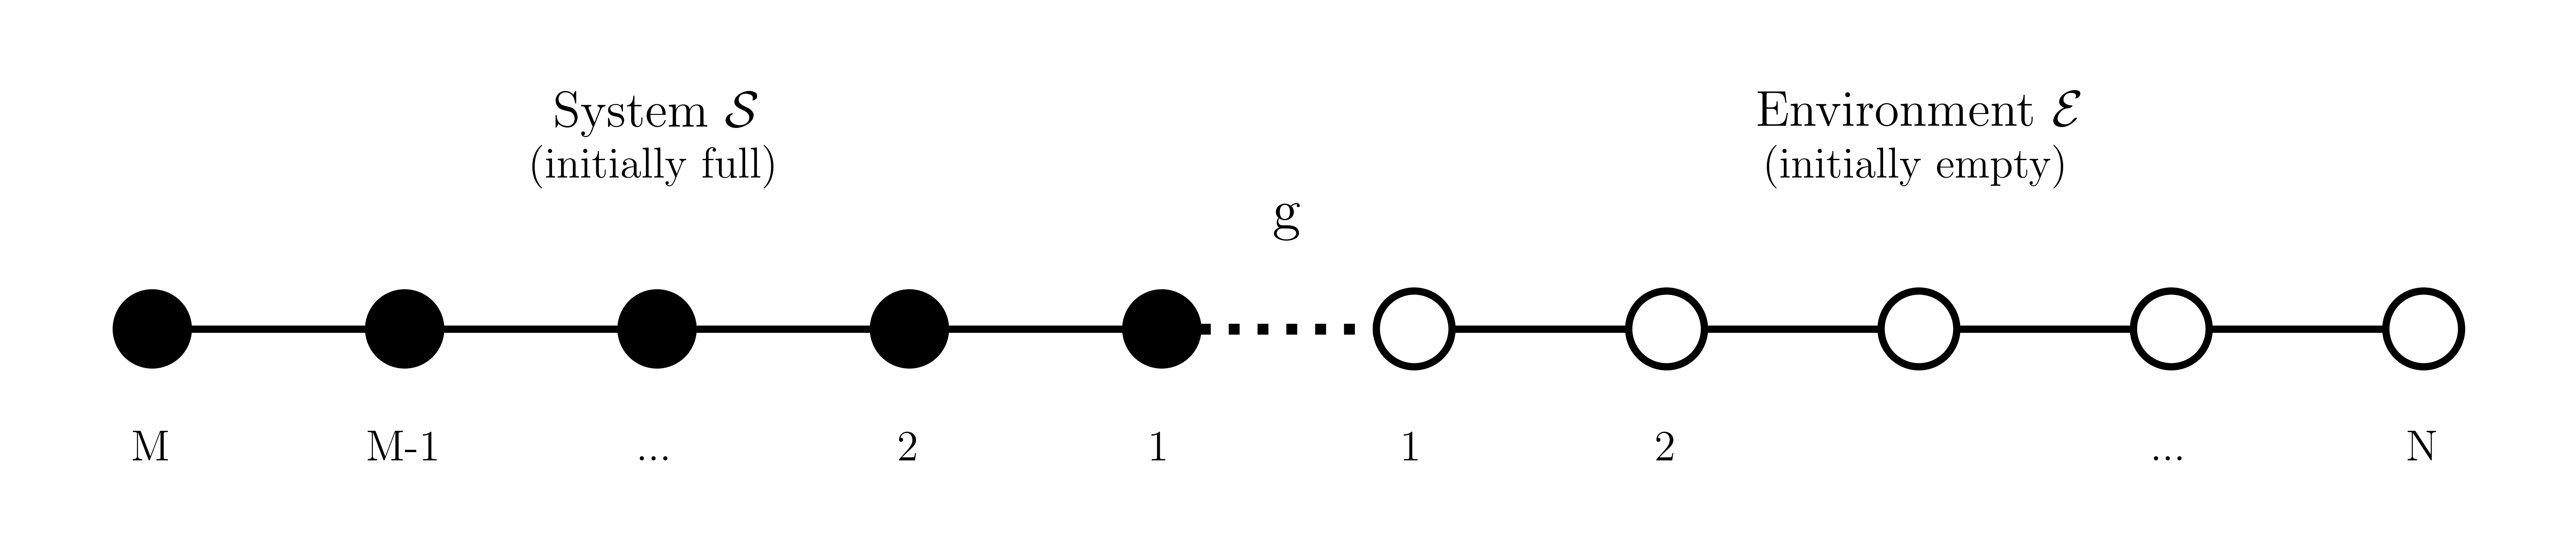
\includegraphics[width=0.65\textwidth]{figures/fermion_model_diagram.png}
    \end{center}
    
    \vspace{-0.5cm}
    
    \begin{columns}
        \begin{column}{0.5\textwidth}
            \textbf{System} ($M$ sites, initially full):
            \begin{equation*}
                H_{\mathrm{sys}} = -t_{\mathrm{sys}} \sum_{i=1}^{M-1} (c_i^\dagger c_{i+1} + \text{h.c.})
            \end{equation*}
        \end{column}
        \begin{column}{0.5\textwidth}
            \textbf{Environment} ($N \gg M$ sites, initially empty):
            \begin{equation*}
                H_{\mathrm{env}} = -t_{\mathrm{env}} \sum_{j=1}^{N-1} (f_j^\dagger f_{j+1} + \text{h.c.})
            \end{equation*}
        \end{column}
    \end{columns}
    
    \vspace{0.1cm}

    \textbf{Boundary coupling:} $H_c = g(c_1^\dagger f_1 + f_1^\dagger c_1)$, \quad $g \ll t_{\mathrm{sys}},\, t_{\mathrm{env}}$\\
    \textbf{Initial state:} $|\Psi(0)\rangle = \prod_{i=1}^M c_i^\dagger |\Omega\rangle$ \quad (system full, environment empty)

    {\footnotesize Full return of $S_{\mathrm{vN}}(t)$ to zero requires $N \gg M^2$.}
\end{frame}

\begin{frame}{Why Page Curve is Expected}
    \begin{columns}
        \begin{column}{0.55\textwidth}
            \begin{itemize}
                \item \textbf{Early times:} tunneling creates system-environment entanglement, so $S_{\mathrm{vN}}$ increases.
                \item \textbf{Intermediate times:} effective subsystem dimension
                \[
                \dim \Hsys^{\mathrm{(eff)}} = \binom{M}{m(t)}
                \]
                is largest near $m(t)\approx M/2$.
                \item \textbf{Late times:} as the subsystem empties, $\dim \Hsys^{\mathrm{(eff)}} \to 1$, so $S_{\mathrm{vN}} \to 0$.
            \end{itemize}
        \end{column}
        \begin{column}{0.45\textwidth}
            \begin{center}
                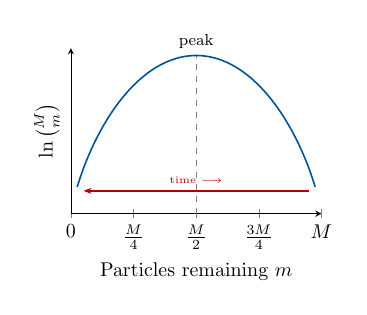
\begin{tikzpicture}[scale=0.72]
                    \begin{axis}[
                        xlabel={Particles remaining $m$},
                        ylabel={$\ln\binom{M}{m}$},
                        xmin=0, xmax=20,
                        ymin=0, ymax=14.5,
                        axis lines=left,
                        width=6cm,
                        height=4.5cm,
                        xtick={0,5,10,15,20},
                        xticklabels={$0$,$\frac{M}{4}$,$\frac{M}{2}$,$\frac{3M}{4}$,$M$},
                        ytick=\empty,
                        clip=false,
                        every axis plot/.append style={thick},
                    ]
                    % Binomial coefficient curve via Stirling: m ln(M/m) + (M-m) ln(M/(M-m))
                    \addplot[thick, iubblue, smooth, samples=200, domain=0.5:19.5]
                        {x*ln(20/x) + (20-x)*ln(20/(20-x))};
                    % Peak annotation
                    \draw[dashed, gray] (axis cs:10,0) -- (axis cs:10,13.86);
                    \node[above, font=\footnotesize] at (axis cs:10,13.86) {peak};
                    % Arrow showing time direction
                    \draw[-{Stealth[length=4pt]}, red!70!black, thick] 
                        (axis cs:19,2) -- (axis cs:1,2);
                    \node[font=\tiny, red!70!black, above] at (axis cs:10,2) {time $\longrightarrow$};
                    \end{axis}
                \end{tikzpicture}\\[2pt]
                {\footnotesize Entropy bounded by $\ln\binom{M}{m}$:}\\
                {\footnotesize rises, peaks at half-filling, falls.}
            \end{center}
        \end{column}
    \end{columns}
\end{frame}

%=============================================================================
\section{Analytical Solution}
%=============================================================================

\begin{frame}{Diagonalizing the System Hamiltonian}
\small
    \textbf{Step 1:} Solve the discrete Schr\"odinger equation with open boundary conditions.

    \vspace{-0.1cm}
    \textbf{System eigenvalues} (single-particle energies):
    \[
        \omega_k = -2t_{\mathrm{sys}}\cos\!\left(\frac{\pi k}{M+1}\right), \quad k = 1,\ldots,M
    \]

    \textbf{Eigenfunctions} (momentum modes):
    \[
        \psi_k(i) = \sqrt{\frac{2}{M+1}}\sin\!\left(\frac{\pi k i}{M+1}\right)
    \]

    \textbf{Step 2:} Express coupling in the diagonal basis via $c_1 = \sum_k \psi_k(1)\, c_k$:
    \[
        H_c = \sum_{k=1}^M V_k(c_k^\dagger f_1 + f_1^\dagger c_k), \qquad V_k = g\sqrt{\frac{2}{M+1}}\sin\!\left(\frac{\pi k}{M+1}\right)
    \]
    \vspace{-0.3cm}

    Each mode $k$ now couples \emph{independently} to the environment boundary site.
\end{frame}

\begin{frame}{Decay Rates from Fermi's Golden Rule}
\small
    \textbf{Environment boundary DOS} (semi-infinite chain, Dyson equation):
    \[
        \rho_{\mathrm{loc}}(E) = \frac{\sqrt{4t_{\mathrm{env}}^2 - E^2}}{2\pi\, t_{\mathrm{env}}^2}, \qquad \rho_{\mathrm{loc}}(0) = \frac{1}{\pi t_{\mathrm{env}}}
    \]

    \textbf{Fermi's golden rule} $\to$ decay width of mode $k$:
    $\Gamma_k = 2\pi\,\rho_{\mathrm{loc}}(\omega_k)\,|V_k|^2$

    \textbf{Wide-band (Markov) approximation:} $\rho_{\mathrm{loc}}(E) \approx \rho_{\mathrm{loc}}(0)$
    \[
        \boxed{\Gamma_k = \frac{4g^2}{(M+1)\,t_{\mathrm{env}}} \sin^2\!\left(\frac{\pi k}{M+1}\right)}
    \]

    \begin{itemize}\setlength{\itemsep}{1pt}
        \item \textbf{Born approximation:} $g \ll t_{\mathrm{sys}}, t_{\mathrm{env}}$ (perturbative coupling)
        \item \textbf{Markov approximation:} local DOS slowly varying $\Rightarrow$ energy-independent self-energy
    \end{itemize}
\end{frame}

\begin{frame}{Resonant Level Model Factorization}
\small
    \begin{columns}
        \begin{column}{0.58\textwidth}
            \textbf{Factorization condition:}
            $|\omega_{k+1}-\omega_k| \gg \Gamma_k$ $\Longleftrightarrow$ $g \ll \sqrt{t_{\mathrm{sys}} t_{\mathrm{env}}}$

            \vspace{-0.1cm}
            \textbf{Factorized reduced state:}
            $\rho_{\mathrm{sys}}(t) = \bigotimes_{k=1}^M \rho_k^{(\mathrm{RLM})}(t)$, \; $\rho_k = \begin{pmatrix} n_k & 0 \\ 0 & 1{-}n_k \end{pmatrix}$

            \vspace{0.1cm}
            \textbf{Exact exponential decay:} $n_k(t) = e^{-\Gamma_k t}$

            \vspace{0.1cm}
            \textbf{Entropy} (sum of binary entropies):
            \[
                S^{(\mathrm{vN})} = -\sum_{k=1}^M \Big[n_k\ln n_k + (1{-}n_k)\ln(1{-}n_k)\Big]
            \]
            \vspace{-0.3cm}
            {\footnotesize Refs.~\cite{PhysRevB.32.4410,Langreth1991,Kehrein_2024}}
        \end{column}
        \begin{column}{0.42\textwidth}
            \begin{center}
                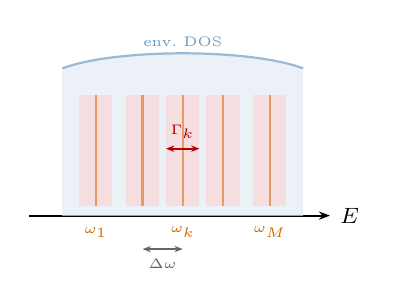
\begin{tikzpicture}[scale=0.85]
                    % Energy axis
                    \draw[-{Stealth[length=4pt]}, thick] (-0.3,0) -- (4.2,0) node[right, font=\footnotesize] {$E$};
                    % DOS background (light fill)
                    \fill[iubblue!8] (0.2,0) -- (0.2,2.2) 
                        .. controls (1,2.5) and (3,2.5) .. (3.8,2.2) 
                        -- (3.8,0) -- cycle;
                    \draw[iubblue!40, thick] (0.2,2.2) 
                        .. controls (1,2.5) and (3,2.5) .. (3.8,2.2);
                    \node[font=\tiny, iubblue!60] at (2,2.6) {env.\ DOS};
                    % System levels with broadening
                    \foreach \x/\lab in {0.7/1, 1.4/2, 2.0/3, 2.6/4, 3.3/5} {
                        \draw[thick, orange!80!black] (\x, 0.15) -- (\x, 1.8);
                        \fill[red!20, opacity=0.5] (\x-0.25, 0.15) rectangle (\x+0.25, 1.8);
                    }
                    % Labels
                    \node[font=\tiny, orange!80!black] at (0.7, -0.25) {$\omega_1$};
                    \node[font=\tiny, orange!80!black] at (2.0, -0.25) {$\omega_k$};
                    \node[font=\tiny, orange!80!black] at (3.3, -0.25) {$\omega_M$};
                    % Broadening annotation
                    \draw[{Stealth[length=3pt]}-{Stealth[length=3pt]}, red!70!black, thick] 
                        (1.75, 1.0) -- (2.25, 1.0);
                    \node[font=\tiny, red!70!black, above] at (2.0, 1.0) {$\Gamma_k$};
                    % Spacing annotation
                    \draw[{Stealth[length=3pt]}-{Stealth[length=3pt]}, black!60, thick] 
                        (1.4, -0.5) -- (2.0, -0.5);
                    \node[font=\tiny, black!60, below] at (1.7, -0.5) {$\Delta\omega$};
                \end{tikzpicture}\\[2pt]
                {\footnotesize $\Delta\omega \gg \Gamma_k$: disjoint windows.}
            \end{center}
        \end{column}
    \end{columns}
\end{frame}

\begin{frame}{Continuum Limit and Universal Form}
\small
    \textbf{Dimensionless time:}
    $\tau = \frac{4g^2}{(M+1)\,t_{\mathrm{env}}}\, t$ \quad (absorbs all model parameters)

    \textbf{Continuum limit} ($M \gg 1$, $q = \pi k/(M{+}1)$):
    \[
        \boxed{n(q, \tau) = e^{-\tau \sin^2 q}, \quad q \in [0, \pi]}
    \]

    \textbf{Entropy per site:}
    $\displaystyle\frac{S(\tau)}{M} = \frac{1}{\pi}\int_0^\pi \!\Big[-n\ln n - (1{-}n)\ln(1{-}n)\Big]\,dq$

    \textbf{Key results:}
    \begin{itemize}\setlength{\itemsep}{1pt}
        \item \textbf{Page time:} $\tau_P \approx 1.16$; physical: $t_P = \tau_P\cdot(M{+}1)t_{\mathrm{env}}/(4g^2) \propto M$
        \item Maximum entropy: $S_{\max} \approx 0.52\,M$
        \item \alert{Universal}: independent of specific values of $M$, $g$, $t_{\mathrm{env}}$
    \end{itemize}
\end{frame}

%=============================================================================
\section{Numerical Method}
%=============================================================================

\begin{frame}{Correlation Matrix Evolution}
\small
    \textbf{Single-particle Hamiltonian} $(M{+}N) \times (M{+}N)$ tridiagonal matrix:
    \[
        h = \begin{pmatrix}
            H_{\mathrm{sys}} & g\,\mathbf{e}_1 \mathbf{e}_1^T \\
            g\,\mathbf{e}_1 \mathbf{e}_1^T & H_{\mathrm{env}}
        \end{pmatrix}
    \]

    \textbf{Diagonalize once:} $h = V D V^\dagger$ $\Longrightarrow$ $U(t) = V e^{-iDt} V^\dagger$

    \textbf{Initial correlation matrix:}
    $\hat{C}(0) = \mathrm{diag}(\mathbb{I}_M,\, 0_N)$ \quad (system full, environment empty)

    \textbf{Time evolution:}
    $\hat{C}(t) = U(t)\,\hat{C}(0)\,U^\dagger(t)$

    \textbf{Extract system block:}
    $C_{\mathcal{S}}(t) = \big[\hat{C}(t)\big]_{1:M,\;1:M}$

    {\footnotesize This is exact --- no approximations beyond finite $N$.}
\end{frame}

\begin{frame}{From Correlation Matrix to Entropy}
    \begin{center}
    \resizebox{0.95\textwidth}{!}{%
    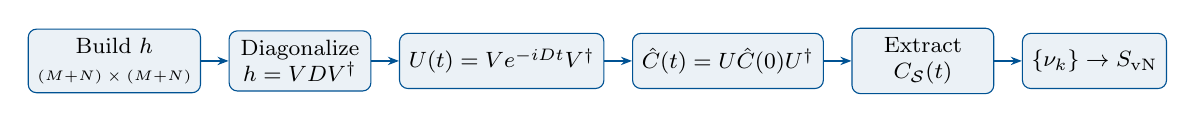
\begin{tikzpicture}[
        box/.style={draw=iubblue, fill=iubblue!8, rounded corners=3pt, 
                     minimum width=1.8cm, minimum height=0.7cm, align=center, font=\footnotesize},
        arr/.style={-{Stealth[length=4pt]}, thick, iubblue},
        node distance=0.35cm
    ]
    \node[box] (h) {Build $h$\\{\tiny $(M{+}N)\times(M{+}N)$}};
    \node[box, right=of h] (diag) {Diagonalize\\$h = VDV^\dagger$};
    \node[box, right=of diag] (prop) {$U(t) = Ve^{-iDt}V^\dagger$};
    \node[box, right=of prop] (evolve) {$\hat{C}(t) = U\hat{C}(0)U^\dagger$};
    \node[box, right=of evolve] (extract) {Extract\\$C_{\mathcal{S}}(t)$};
    \node[box, right=of extract] (ent) {$\{\nu_k\} \to S_{\mathrm{vN}}$};
    
    \draw[arr] (h) -- (diag);
    \draw[arr] (diag) -- (prop);
    \draw[arr] (prop) -- (evolve);
    \draw[arr] (evolve) -- (extract);
    \draw[arr] (extract) -- (ent);
    \end{tikzpicture}%
    }
    \end{center}

    \vspace{0.15cm}
    \textbf{Eigenvalues} $\nu_k \in [0,1]$ of $C_{\mathcal{S}}(t)$ are effective occupations:
    \begin{itemize}
        \item $\nu_k = 0$ or $1$: mode is definitely empty/full $\to$ no entropy
        \item $\nu_k = 0.5$: maximally uncertain $\to$ maximum entropy contribution
    \end{itemize}

    \vspace{0.15cm}
    \textbf{Additional observables} from the same $C_{\mathcal{S}}$:
    \begin{columns}
        \begin{column}{0.5\textwidth}
            \begin{itemize}
                \item Particle number: $m(t) = \Tr C_{\mathcal{S}}(t)$
                \item R\'enyi entropies: $S_\alpha$
            \end{itemize}
        \end{column}
        \begin{column}{0.5\textwidth}
            \textbf{Complexity comparison:}
            \begin{itemize}
                \item Full: $2^M \times 2^M$
                \item Peschel: $M \times M$
                \item Cost: $O(N^3)$ one-time
            \end{itemize}
        \end{column}
    \end{columns}
\end{frame}

%=============================================================================
\section{Results}
%=============================================================================

\begin{frame}{Particle Number Decay}
    \begin{columns}
        \begin{column}{0.45\textwidth}
            \textbf{What we see (Fig.~3):}
            \begin{itemize}\setlength{\itemsep}{1pt}
                \item Smooth exponential decay
                \item \alert{No visible kink at Page time}
            \end{itemize}
            
            \vspace{0.15cm}
            
            \textbf{Implication:}
            \begin{itemize}\setlength{\itemsep}{1pt}
                \item Page curve is a nonlocal information effect
                \item Local observables alone ($I(t) = \dot{m}(t)$) do not reveal turnover
                \item \textbf{Semiclassical breakdown}: current continues smoothly even as entropy drops
            \end{itemize}
        \end{column}
        \begin{column}{0.55\textwidth}
            \begin{center}
                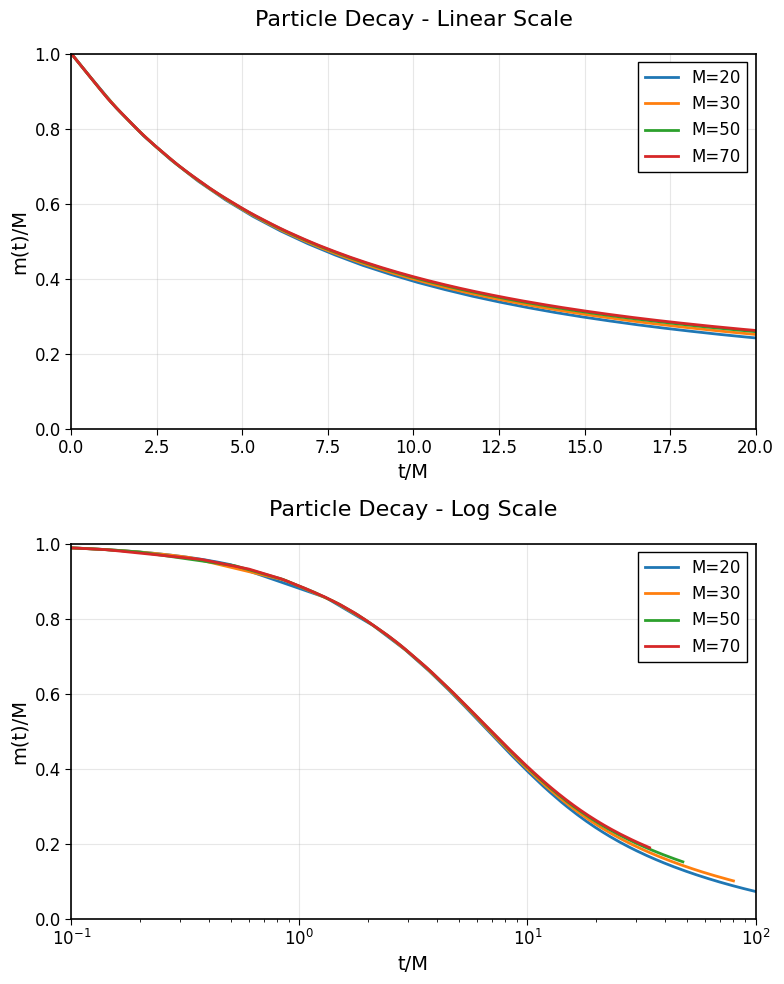
\includegraphics[width=0.73\textwidth,keepaspectratio]{figures/Fig-3.png}
            \end{center}
        \end{column}
    \end{columns}
\end{frame}

\begin{frame}{The Page Curve}
    \begin{columns}
        \begin{column}{0.45\textwidth}
            \textbf{Three regimes:}
            \begin{enumerate}
                \item \textbf{Linear growth} (early times)
                \item \textbf{Maximum} at Page time $t_P \propto M$
                \item \textbf{Decay} to zero (late times)
            \end{enumerate}
            
            \vspace{0.3cm}
            
            \textbf{Key results:}
            \begin{equation*}
                S_{\mathrm{max}} \approx 0.52\, M, \quad \tau_P \approx 1.16
            \end{equation*}
            
            \footnotesize
            Compare with random-state bound $M\ln 2 \approx 0.69M$.\\
            \alert{Free-fermion dynamics: Gaussian, not fully ergodic.}
            \\
            Ref.~\cite{Kehrein_2024}
        \end{column}
        \begin{column}{0.55\textwidth}
            \begin{center}
                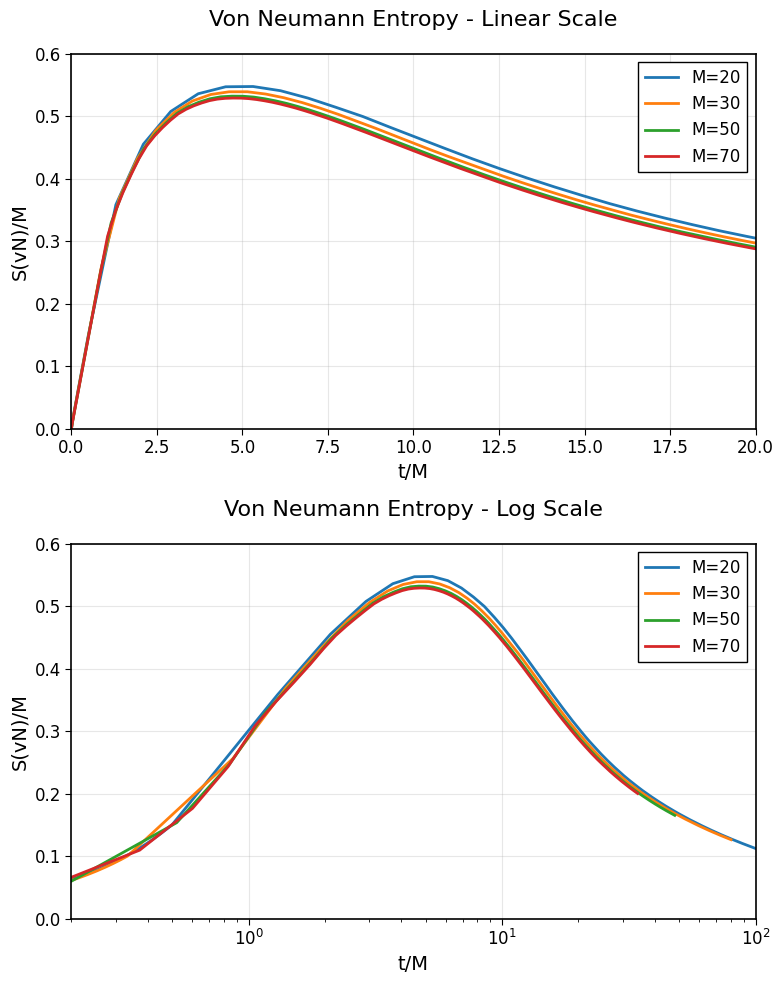
\includegraphics[width=0.73\textwidth,keepaspectratio]{figures/Fig-4.png}
            \end{center}
        \end{column}
    \end{columns}
\end{frame}

\begin{frame}{Universal Scaling Collapse}
    \begin{columns}
        \begin{column}{0.4\textwidth}
            \textbf{Universal behavior:}
            \begin{itemize}
                \item Plot $S$ vs.\ emitted fraction
                \item Weak-coupling curves collapse
                \item Dashed line: analytical RLM
            \end{itemize}
            
            \vspace{0.3cm}
            
            \textbf{Finite-size effects:}
            \begin{itemize}
                \item Deviations at large $g$
                \item Finite bath density of states
                \item Late-time recurrences/reflections
                \item Scaling controlled by $N/M^2$
            \end{itemize}
        \end{column}
        \begin{column}{0.6\textwidth}
            \begin{center}
                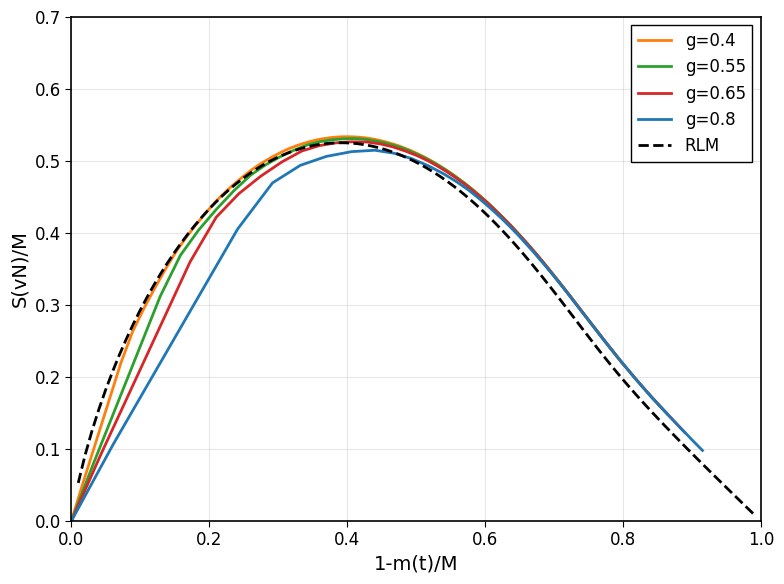
\includegraphics[width=\textwidth]{figures/Fig-5.png}
            \end{center}
        \end{column}
    \end{columns}
\end{frame}

%=============================================================================
\section{Interpretation}
%=============================================================================

\begin{frame}{Physical Interpretation}
    \begin{columns}
        \begin{column}{0.55\textwidth}
            \textbf{System viewpoint:}
            \begin{itemize}
                \item System empties $\Rightarrow$ effective Hilbert space shrinks
                \item Entropy bounded by $\ln(\dim \Hsys^{\mathrm{(eff)}})$
            \end{itemize}

            \vspace{0.2cm}

            \textbf{Environment viewpoint (Observer Paradox):}
            \begin{itemize}
                \item Particles keep arriving while entropy eventually decreases
                \item Late emissions carry correlations that reduce total entanglement
                \item Robust and reproducible --- not fine-tuned
            \end{itemize}
        \end{column}
        \begin{column}{0.45\textwidth}
            \begin{center}
                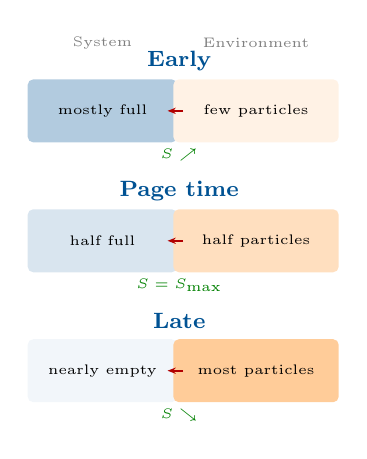
\begin{tikzpicture}[scale=0.75,
                    sysbox/.style={thick, rounded corners=2pt, minimum width=1.9cm, minimum height=0.8cm, inner sep=2pt, font=\tiny, align=center},
                    envbox/.style={thick, rounded corners=2pt, minimum width=2.1cm, minimum height=0.8cm, inner sep=2pt, font=\tiny, align=center}]
                    % Three stages
                    \def\sy{0.0}
                    % Stage 1: Early
                    \node[font=\footnotesize\bfseries, iubblue] at (2.1, \sy+3.0) {Early};
                    \node[sysbox, fill=iubblue!30] (s1) at (0.8, \sy+2.15) {mostly full};
                    \node[envbox, fill=orange!10] (e1) at (3.4, \sy+2.15) {few particles};
                    \draw[-{Stealth[length=3pt]}, thick, red!70!black] (s1.east) ++(0.08,0) -- ($(e1.west)+(-0.08,0)$);
                    \node[font=\tiny, green!50!black] at (2.1, \sy+1.4) {$S \nearrow$};

                    % Stage 2: Page time
                    \def\sy{-2.2}
                    \node[font=\footnotesize\bfseries, iubblue] at (2.1, \sy+3.0) {Page time};
                    \node[sysbox, fill=iubblue!15] (s2) at (0.8, \sy+2.15) {half full};
                    \node[envbox, fill=orange!25] (e2) at (3.4, \sy+2.15) {half particles};
                    \draw[-{Stealth[length=3pt]}, thick, red!70!black] (s2.east) ++(0.08,0) -- ($(e2.west)+(-0.08,0)$);
                    \node[font=\tiny, green!50!black] at (2.1, \sy+1.4) {$S = S_{\max}$};

                    % Stage 3: Late
                    \def\sy{-4.4}
                    \node[font=\footnotesize\bfseries, iubblue] at (2.1, \sy+3.0) {Late};
                    \node[sysbox, fill=iubblue!5] (s3) at (0.8, \sy+2.15) {nearly empty};
                    \node[envbox, fill=orange!40] (e3) at (3.4, \sy+2.15) {most particles};
                    \draw[-{Stealth[length=3pt]}, thick, red!70!black] (s3.east) ++(0.08,0) -- ($(e3.west)+(-0.08,0)$);
                    \node[font=\tiny, green!50!black] at (2.1, \sy+1.4) {$S \searrow$};

                    % System/Env labels at top
                    \node[font=\tiny, gray] at (0.8, 3.3) {System};
                    \node[font=\tiny, gray] at (3.4, 3.3) {Environment};
                \end{tikzpicture}
            \end{center}
        \end{column}
    \end{columns}

    \vspace{0.1cm}
    \textbf{Key message:} rise-and-fall is a generic feature of weak-coupling unitary dynamics.
\end{frame}

\begin{frame}{Scope \& Limitations}
    \textbf{Regime of validity:}
    \begin{itemize}
        \item Weak coupling: $g \ll t_{\mathrm{sys}},\, t_{\mathrm{env}}$
        \item Broad-band environment: $t_{\mathrm{env}} \gtrsim t_{\mathrm{sys}}$ (we use $t_{\mathrm{env}} = 4\,t_{\mathrm{sys}}$)
        \item Large environment: $N \gg M^2$ for full Page curve
    \end{itemize}

    \vspace{0.3cm}
    \textbf{What this model does \emph{not} capture:}
    \begin{itemize}
        \item Interactions between fermions (non-Gaussian correlations)
        \item Finite-temperature initial states
        \item Band-edge mode corrections (small fraction of modes near $\omega \approx \pm 2t_{\mathrm{sys}}$)
    \end{itemize}

    \vspace{0.3cm}
    \textbf{Simulation parameters:} $M = 10$--$100$ sites, $N = 10\,000$, $g/t_{\mathrm{sys}} = 0.05$--$0.65$
\end{frame}

%=============================================================================
\section{Conclusions}
%=============================================================================

\begin{frame}{Summary}
\small
    \textbf{Main achievements:}
    \begin{enumerate}\setlength{\itemsep}{0pt}
        \item Showed \alert{Page-curve-like} entanglement dynamics in an open free-fermion chain
        \item Derived analytical dynamics via resonant level model factorization
        \item Validated predictions numerically using correlation matrices
        \item Found universal scaling with dimensionless time/emitted fraction
    \end{enumerate}
    
    \textbf{Physical insights:}
    \begin{itemize}\setlength{\itemsep}{0pt}
        \item Local currents do not signal the Page-time turnover
        \item Entanglement controlled by effective Hilbert-space reduction
        \item Rise-and-fall driven by shrinking effective Hilbert space as system empties
    \end{itemize}
\end{frame}

\begin{frame}{Future Directions}
    \begin{itemize}
        \item \textbf{Bosonic systems:} Coupled harmonic oscillators
        \item \textbf{Interacting models:} Beyond quadratic Hamiltonians
        \item \textbf{Different geometries:} Bulk and multi-contact coupling
        \item \textbf{Finite temperature:} Thermal initial baths
        \item \textbf{Experiments:} Quantum gas microscopes in optical lattices with single-site resolution
    \end{itemize}
    
    \vspace{0.5cm}
    
    \begin{center}
        \textbf{Core mechanism:}\\
        Entanglement rises during emission and falls as the subsystem's effective state space collapses.
    \end{center}
\end{frame}

% Main talk endpoint
\begin{frame}
    \centering
    \Huge Thank You!
    
    \vspace{0.6cm}
    
    \Large Questions?
    
    \vspace{0.6cm}
    
    \normalsize
    \texttt{2010271@iub.edu.bd}
    
    \vspace{0.4cm}
    \small
    \textit{Free-fermion chains exhibit universal Page-curve dynamics\\controlled by effective Hilbert-space reduction.}
    
    \vspace{0.3cm}
    \footnotesize
    \textit{We thank the Center for Computational \& Data Sciences (CCDS), IUB,\\for providing the computational resources used in this work.}
\end{frame}

%=============================================================================
% Appendix (backup + references)
%=============================================================================
\appendix
\section*{Backup}

\begin{frame}{Backup: Bell State Derivation}
\small
    \textbf{State:} $\ket{\Psi} = \tfrac{1}{\sqrt{2}}\big(\ket{0}_A\ket{1}_B + \ket{1}_A\ket{0}_B\big)$

    \textbf{Density matrix} $\rho_{AB} = \ket{\Psi}\bra{\Psi}$:
    \[
        \rho_{AB} = \tfrac{1}{2}\Big(\ket{01}\bra{01} + \ket{01}\bra{10} + \ket{10}\bra{01} + \ket{10}\bra{10}\Big)
    \]

    \textbf{Partial trace over $B$} \quad ($\rho_A = \sum_{b=0,1} \bra{b}_B\,\rho_{AB}\,\ket{b}_B$):
    \begin{align*}
        \bra{0}_B\,\rho_{AB}\,\ket{0}_B &= \tfrac{1}{2}\ket{1}_A\bra{1}_A \\
        \bra{1}_B\,\rho_{AB}\,\ket{1}_B &= \tfrac{1}{2}\ket{0}_A\bra{0}_A
    \end{align*}
    \[
        \boxed{\rho_A = \tfrac{1}{2}\ket{0}\bra{0} + \tfrac{1}{2}\ket{1}\bra{1} = \tfrac{1}{2}\mathbb{I}_A}
    \]

    \textbf{Entanglement entropy:}
    Eigenvalues of $\rho_A$: $p_1 = p_2 = \tfrac{1}{2}$
    \[
        S_A = -\sum_i p_i \ln p_i = -2 \cdot \tfrac{1}{2}\ln\tfrac{1}{2} = \ln 2 \approx 0.693
    \]
    Maximally entangled: $S_A = \ln d_A = \ln 2$ \checkmark \quad $\Tr(\rho_A^2) = \tfrac{1}{2} < 1$ (mixed) \checkmark
\end{frame}

\begin{frame}{Backup: Second Quantization}
    \textbf{Fermionic operators:}
    \begin{align*}
        \{c_i, c_j^\dagger\} &= \delta_{ij} \\
        \{c_i, c_j\} &= \{c_i^\dagger, c_j^\dagger\} = 0
    \end{align*}
    
    \textbf{Hamiltonian in diagonal form:}
    \begin{equation*}
        H = \sum_{k=1}^M \omega_k c_k^\dagger c_k + \sum_{k=1}^M V_k(c_k^\dagger f_1 + f_1^\dagger c_k) + H_{\mathrm{env}}
    \end{equation*}
    
    \textbf{Initial state:}
    \begin{equation*}
        \ket{\Psi(0)} = \prod_{i=1}^M c_i^\dagger \ket{\Omega} = \prod_{k=1}^M c_k^\dagger \ket{\Omega}
    \end{equation*}
\end{frame}

\begin{frame}{Backup: 2-Site Toy Model Numerics ($M=2, N=1$)}
    \begin{columns}
        \begin{column}{0.45\textwidth}
            \textbf{Single-particle Hamiltonian $h$:}
            \begin{equation*}
            h = \begin{pmatrix}
            0 & -t_{\mathrm{sys}} & -g \\
            -t_{\mathrm{sys}} & 0 & 0 \\
            -g & 0 & 0
            \end{pmatrix}
            \end{equation*}
            {\footnotesize Basis: $(c_1, c_2, f_1)$}
            
            \vspace{0.3cm}
            \textbf{Evolution:}
            $U(t) = e^{-iht}$
        \end{column}
        \begin{column}{0.55\textwidth}
            \textbf{Correlation Matrix $\hat{C}$:}
            \begin{equation*}
            \hat{C}(0) = \begin{pmatrix}
            1 & 0 & 0 \\
            0 & 1 & 0 \\
            0 & 0 & 0
            \end{pmatrix} \rightarrow \hat{C}(t) = U(t) \hat{C}(0) U^\dagger(t)
            \end{equation*}
            
            \vspace{0.1cm}
            \textbf{Subsystem Block:}
            \begin{equation*}
            C_{\mathcal{S}}(t) = \begin{pmatrix}
            \hat{C}_{11}(t) & \hat{C}_{12}(t) \\
            \hat{C}_{21}(t) & \hat{C}_{22}(t)
            \end{pmatrix}
            \end{equation*}
            {\footnotesize Diagonalize $C_{\mathcal{S}}$ to find $\nu_1, \nu_2$ for $S_{\mathrm{vN}}$.}
        \end{column}
    \end{columns}
\end{frame}

\begin{frame}{Backup: Validity Conditions}
    \textbf{Approximations used:}
    \begin{enumerate}
        \item \textbf{Weak coupling:} $g \ll t_{\mathrm{sys}}, t_{\mathrm{env}}$
        \item \textbf{Broad-band regime:} $t_{\mathrm{env}} \gtrsim t_{\mathrm{sys}}$ (we use $t_{\mathrm{env}}=4\,t_{\mathrm{sys}}$)
        \item \textbf{Mode independence:} $g \ll \sqrt{t_{\mathrm{sys}} t_{\mathrm{env}}}$
        \item \textbf{Large system:} $M \gg 1$ (continuum limit)
        \item \textbf{Large environment:} $N \gg M^2$ (no recurrence)
    \end{enumerate}
    
    \vspace{0.3cm}
    
    \textbf{Time window:} $t \ll N/t_{\mathrm{env}}$ \quad (before finite-size recurrences)
\end{frame}

\begin{frame}{Backup: Effective Hilbert Space Bound}
    At time $t$, approximately $m(t)$ particles remain in system.
    
    \vspace{0.3cm}
    
    \textbf{Effective dimension:}
    \begin{equation*}
        \dim \Hsys^{\mathrm{(eff)}} = \binom{M}{m(t)}
    \end{equation*}
    
    \textbf{Entropy bound} (Stirling approximation):
    \begin{equation*}
        S_{\mathrm{vN}} \lesssim m \ln\frac{M}{m} + (M-m)\ln\frac{M}{M-m}
    \end{equation*}
    
    \begin{itemize}
        \item Maximum at $m = M/2$ (half-filled)
        \item Vanishes as $m \to 0$ or $m \to M$
    \end{itemize}
\end{frame}

\begin{frame}{Backup: Finite-Size Effects}
    \begin{columns}
        \begin{column}{0.45\textwidth}
            \textbf{Environment size $N$:}
            \begin{itemize}
                \item Full Page curve requires $N \gg M^2$
                \item Smaller $N$: entropy doesn't return to zero
                \item Reflections from environment boundary cause recurrences
            \end{itemize}
            
            \vspace{0.3cm}
            
            \textbf{Parameters:}\\
            {\footnotesize $M=50$, $t_{\mathrm{sys}}=t_{\mathrm{env}}=1$, $g=0.65$\\
            $N= 75, 100, 200, 300, 10000$}
        \end{column}
        \begin{column}{0.55\textwidth}
            \begin{center}
                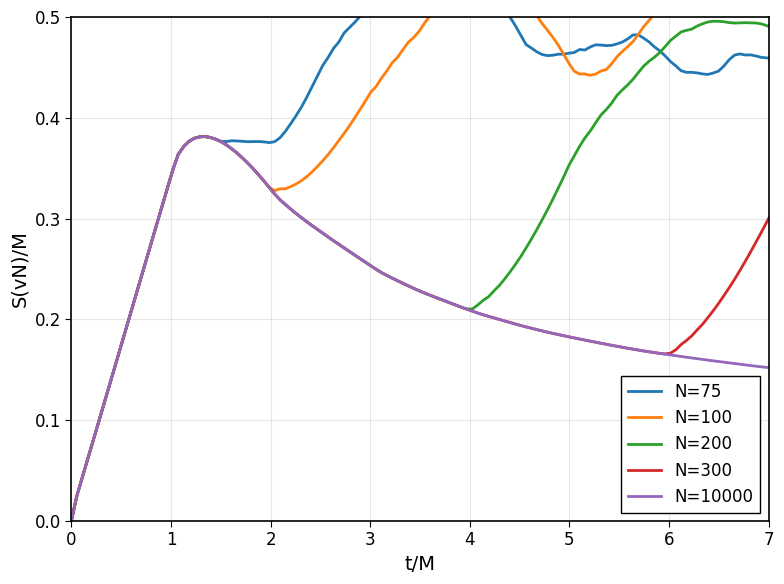
\includegraphics[height=0.57\textheight,keepaspectratio]{figures/Fig-6.png}
            \end{center}
        \end{column}
    \end{columns}
\end{frame}

\begin{frame}{Backup: Connection to Black Holes}
    \begin{columns}
        \begin{column}{0.5\textwidth}
            \textbf{Analogy:}
            \begin{itemize}
                \item System $\mathcal{S}$ $\longleftrightarrow$ black hole interior
                \item Environment $\mathcal{E}$ $\longleftrightarrow$ Hawking radiation
                \item Coupling $g$ $\longleftrightarrow$ horizon transmission
                \item Unitary evolution $\longleftrightarrow$ information preservation
            \end{itemize}
        \end{column}
        \begin{column}{0.5\textwidth}
            \textbf{Key differences:}
            \begin{itemize}
                \item No event horizon or gravity
                \item Free fermions (exactly solvable)
                \item Finite system (not thermodynamic)
            \end{itemize}
            
            \vspace{0.3cm}
            \textbf{``Burning piece of coal''} (Polchinski):\\
            {\footnotesize Early photons entangled with coal; late photons purify the radiation state.}
        \end{column}
    \end{columns}
\end{frame}

\begin{frame}{Backup: Semiclassical Breakdown at Page Time}
    \textbf{Early times:} semiclassical picture holds
    \[
    \frac{dS^{(\mathrm{vN})}}{dt} \propto |I(t)| \quad \text{(each tunneling event} \to \text{entanglement)}
    \]
    
    \vspace{0.3cm}
    
    \textbf{At Page time:} this relation \alert{must break down}
    \begin{itemize}
        \item Particle current $I(t) = \dot{m}(t)$ is smooth --- no kink at $t_P$
        \item Yet entropy turns over and decreases
        \item Late emissions \textit{reduce} entanglement by purifying earlier correlations
    \end{itemize}
    
    \vspace{0.3cm}
    
    \textbf{Conclusion:} the Page curve is a \alert{quantum information} effect, invisible to any local observable.
\end{frame}

\begin{frame}{Backup: Eisler--Peschel Formalism}
    \textbf{Problem:} Computing $S^{(\mathrm{vN})}$ naively requires the many-body density matrix $\rho_{\mathrm{sys}}$ of dimension $2^M \times 2^M$.

    \vspace{0.3cm}

    \textbf{Peschel's key result} \cite{Peschel_2009}: For free fermions, $\rho_{\mathrm{sys}}$ is Gaussian:
    \[
    \rho_{\mathrm{sys}} = K \exp\!\Bigl(-\sum_{i,j=1}^{M} h_{ij}\, c_i^\dagger c_j\Bigr), \qquad h = \ln\!\bigl((1-C)/C\bigr)
    \]
    $\Rightarrow$ \alert{completely determined} by the $M \times M$ correlation matrix $C_{ij}(t) = \langle c_i^\dagger(t)\, c_j(t)\rangle$.

    \vspace{0.3cm}

    \textbf{Entropy from eigenvalues $\{n_k\}$ of $C_{\mathrm{sys}}$:}
    \[
    S^{(\mathrm{vN})} = -\sum_{k=1}^{M}\bigl[n_k \ln n_k + (1{-}n_k)\ln(1{-}n_k)\bigr]
    \]
\end{frame}

\begin{frame}{Backup: Computational Complexity Reduction}
    \begin{columns}[T]
    \begin{column}{0.48\textwidth}
        \textbf{Na\"ive (many-body):}
        \begin{itemize}
            \item State vector: $2^{M+N}$
            \item Diagonalise $\rho_{\mathrm{sys}}$: $O(2^{3M})$
            \item $M{=}75$: \alert{impossible}
        \end{itemize}
    \end{column}
    \begin{column}{0.48\textwidth}
        \textbf{Peschel formalism:}
        \begin{itemize}
            \item Diagonalise $h$: $O((M{+}N)^3)$
            \item Evolve $C(t)$: $O((M{+}N)^2)$/step
            \item $N{=}10^4$: \alert{seconds on a laptop}
        \end{itemize}
    \end{column}
    \end{columns}

    \vspace{0.5cm}
    \centering
    \alert{Exponential $\to$ Polynomial}: the reduction that makes the simulation tractable.
\end{frame}

\section*{References}
\begin{frame}[allowframebreaks]{References}
    \printbibliography[heading=none]
\end{frame}

\end{document}
